\setcounter{exo}{0}
\begin{flushright}
D'après Florestan Mathurin.
\end{flushright}
\ifprof
\else
Soit un système dont le diagramme de Bode est donné ci-dessous.
\begin{center}
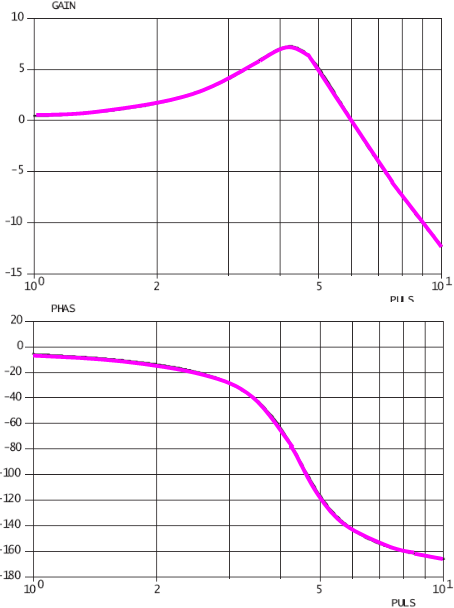
\includegraphics[width=\linewidth]{img_01}
\end{center}


\subparagraph{}
\textit{Tracer le diagramme de Bode asymptotique.}
\ifprof
%\begin{corrige}
%\end{corrige}
\else
\fi


\subparagraph{}
\textit{Identifier le type de la fonction de transfert et ses valeurs remarquables.}


\subparagraph{}
\textit{Le diagramme temporel ci-dessous présente 3 signaux d'entrée sinusoïdaux. Déterminer les période et les pulsations de chacun des signaux. }


\begin{center}
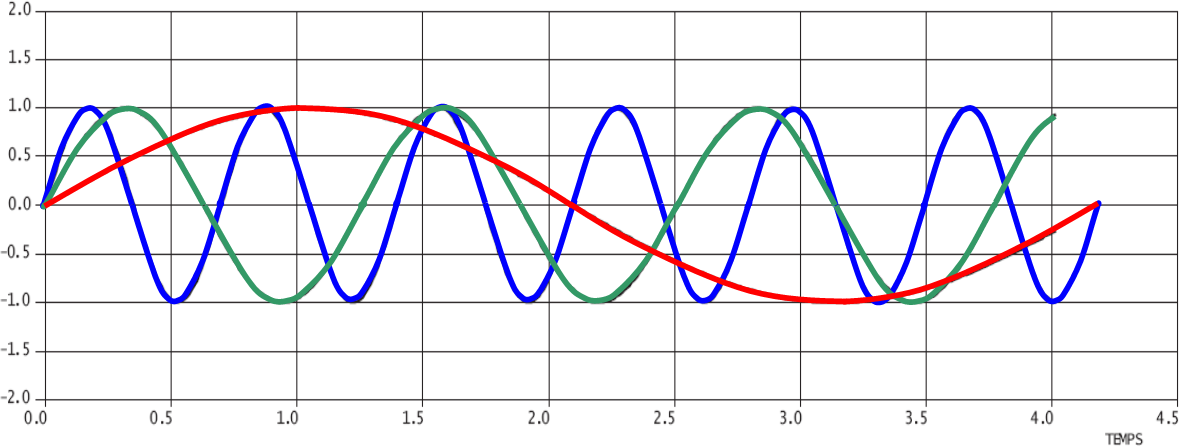
\includegraphics[width=\linewidth]{img_02}
\end{center}


\ifprof
%\begin{corrige}
%\end{corrige}
\else
\fi


\subparagraph{}
\textit{En déduire le gain et le déphasage en régime permanent pour chacune des courbes temporelles de sortie correspondant aux 3 entrées de la question 3. }
\ifprof
%\begin{corrige}
%\end{corrige}
\else
\fi
